\documentclass[]{article}
\usepackage[ ]{indentfirst}
\usepackage{tikz}
\usepackage[ ]{graphicx}
\title{Revisão P1\\Linguagens Formais e Autômatos}
\author{Erickson G. Müller}
\date{}

\begin{document}
	\maketitle
	\section{Conteúdos}
		\begin{enumerate}
			\item Conceitos e linguagens: 
			\begin{itemize}
				\item Símbolo
				\item Alfabeto: conjunto de símbolos (terminais) utilizados para formar cadeias que pertencem a uma linguagem.
				\item Cadeia
				\item Sentença 
				\item Concatenação
				\item Fechamento 
				\item Sufixo
				\item Prefixo
				\item Definição formal de gramática gerativa e derivação
				\item Tipos de gramáticas
			\end{itemize}
			\item Conceitos e linguagens
				Símbolo, alfabeto, cadeia, sentença, concatenação, fechamento, sufixo, prefixo. Definição
		\end{enumerate}
	\section{Teoria de Linguagens}
		\begin{itemize}
			\item Símbolo: qualidade e precedência
			\item Cadeia
			\item Tamanho de cadeia (caso cadeia vazia ($\epsilon$) )%símbolo grego
			\item prefixo (próprio)
			\item sufixo (próprio)
			\item concatenação
			\item fechamento
			\begin{enumerate}
				\item V*
				\item V+ = V* - {EE}
			\end{enumerate}
			\item linguagem finita
			\item linguagem infinita
			\item Reconhecedor: busca identificar se a sentença(ou cadeia, dependendo da apostila vs professor) pertence à linguagem ou não.
			\item sistema gerativo (gramática gerativa)

		\end{itemize}
		Computabilidade; Algoritmos e decibilidade; Soluções algoritmica decidíveis e indecidíveis. Processadores de linguagens (tradutores e interpretadores).
		
		Para problemas computáveis podemos construir uma solução algoritmica que poderá ou não ter um resultado. Caso esse algoritmo não tenha um retorno, será considerado um algoritmo indecidível.
		
		Esse conjunto de cadeias pode ser formado pela concatenação de símbolos que pertence ao alfabeto da linguagem.
		
		Os processadores de linguagem verificam se a cadeia de símbolos \textbf{pertence} à linguagem. Os processadores de linguagens são soluções algoritmicas para \textbf{problemas decidíveis}. São divididos em tradutores e interpretadores.
		
		Símbolos não têm significado intrínsico, a diferença entre eles é pela sua representação gráfica. O símbolo estará sob regras de substituição.
		
		Os processadores de linguagens podem fazer transformações de linguagens de mesmo nível, podem passar de uma linguagem de código de uma máquina para outra máquina.
		
		Tradutores recebem uma entrada chamada de fonte, fazem o processamento e resultam um objeto.
%		\begin{tikzpicture}
%			\node (processo) [draw, ellipse] {processamento};
%			\node (fonte) [left=of processo] {fonte};
%			\node (objeto) [right=of processo] {objeto};
%			\draw [->] (fonte) -- (processo);
%			\draw [->] (processo) -- (objeto);
%		\end{tikzpicture}

		Nem todas as cadeias do fechamento do alfabeto são sentenças, todas as sentenças pertencem ao fechamento do alfabeto
		
		\textbf{Gramática:} Conjunto de regras que descreve como as cadeias podem ser montadas e quando elas são válidas.
		
		Sentença é toda cadeia de símbolos que pertence à linguagem.
		
		Aplicando as regras da gramática, teremos sempre uma \textit{cadeia ou sentença} %não sei qual dos dois
		\begin{center}
		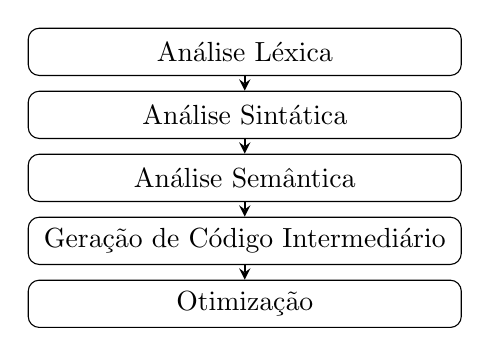
\begin{tikzpicture}[node distance=0.8cm, auto]
\tikzstyle{bloco} = [rectangle, rounded corners, minimum width=5.5cm, minimum height=0.6cm,text centered, draw=black]
\tikzstyle{seta} = [thick,->,>=stealth]

\node [bloco] (lexica) {Análise Léxica};
\node [bloco, below of=lexica] (um) {Análise Sintática};
\node [bloco, below of=um] (dois) {Análise Semântica};
\node [bloco, below of=dois] (tres) {Geração de Código Intermediário};
\node [bloco, below of=tres] (quatro) {Otimização};

\draw [seta] (lexica) -- (um);
\draw [seta] (um) -- (dois);
\draw [seta] (dois) -- (tres);
\draw [seta] (tres) -- (quatro);

\end{tikzpicture}
\end{center}

		Análise léxica faz o tratamento de erros, reconhecimento do tipo da variável através do identificador

		Faz parte da saída da análise léxica uma estrutura chamada de fita que pertence o identificador dos tokens, essa fita é a entrada da análise sintática. O final dessa fita é um símbolo de final de sentença. 

		Análise sintática faz a análise da sentença  usando o identificadores das cadeias que foram validadas na análise léxica. A sentença é avaliada através da concatenação de identificadores em uma determinada ordem.
		
		A análise semântica verifica  o tipo dos siímbolos e como estão sendo utilizados.
		
		A geração de Código intermediário passa a sentença para código assembly.
		
		Concatenação de símbolos de um alfabeto de uma linguagem, essa concatenação vai formar cadeias. Essas cadeias podem ser sentenças ou não. Caso a cadeia pertença à linguagem, é considerado uma sentença.
		
		Fechamento do alfabeto de uma linguagem é a concatenação dos símbolos do alfabeto em qualquer ordem e em qualquer quantidade.
		
		\begin{center}
			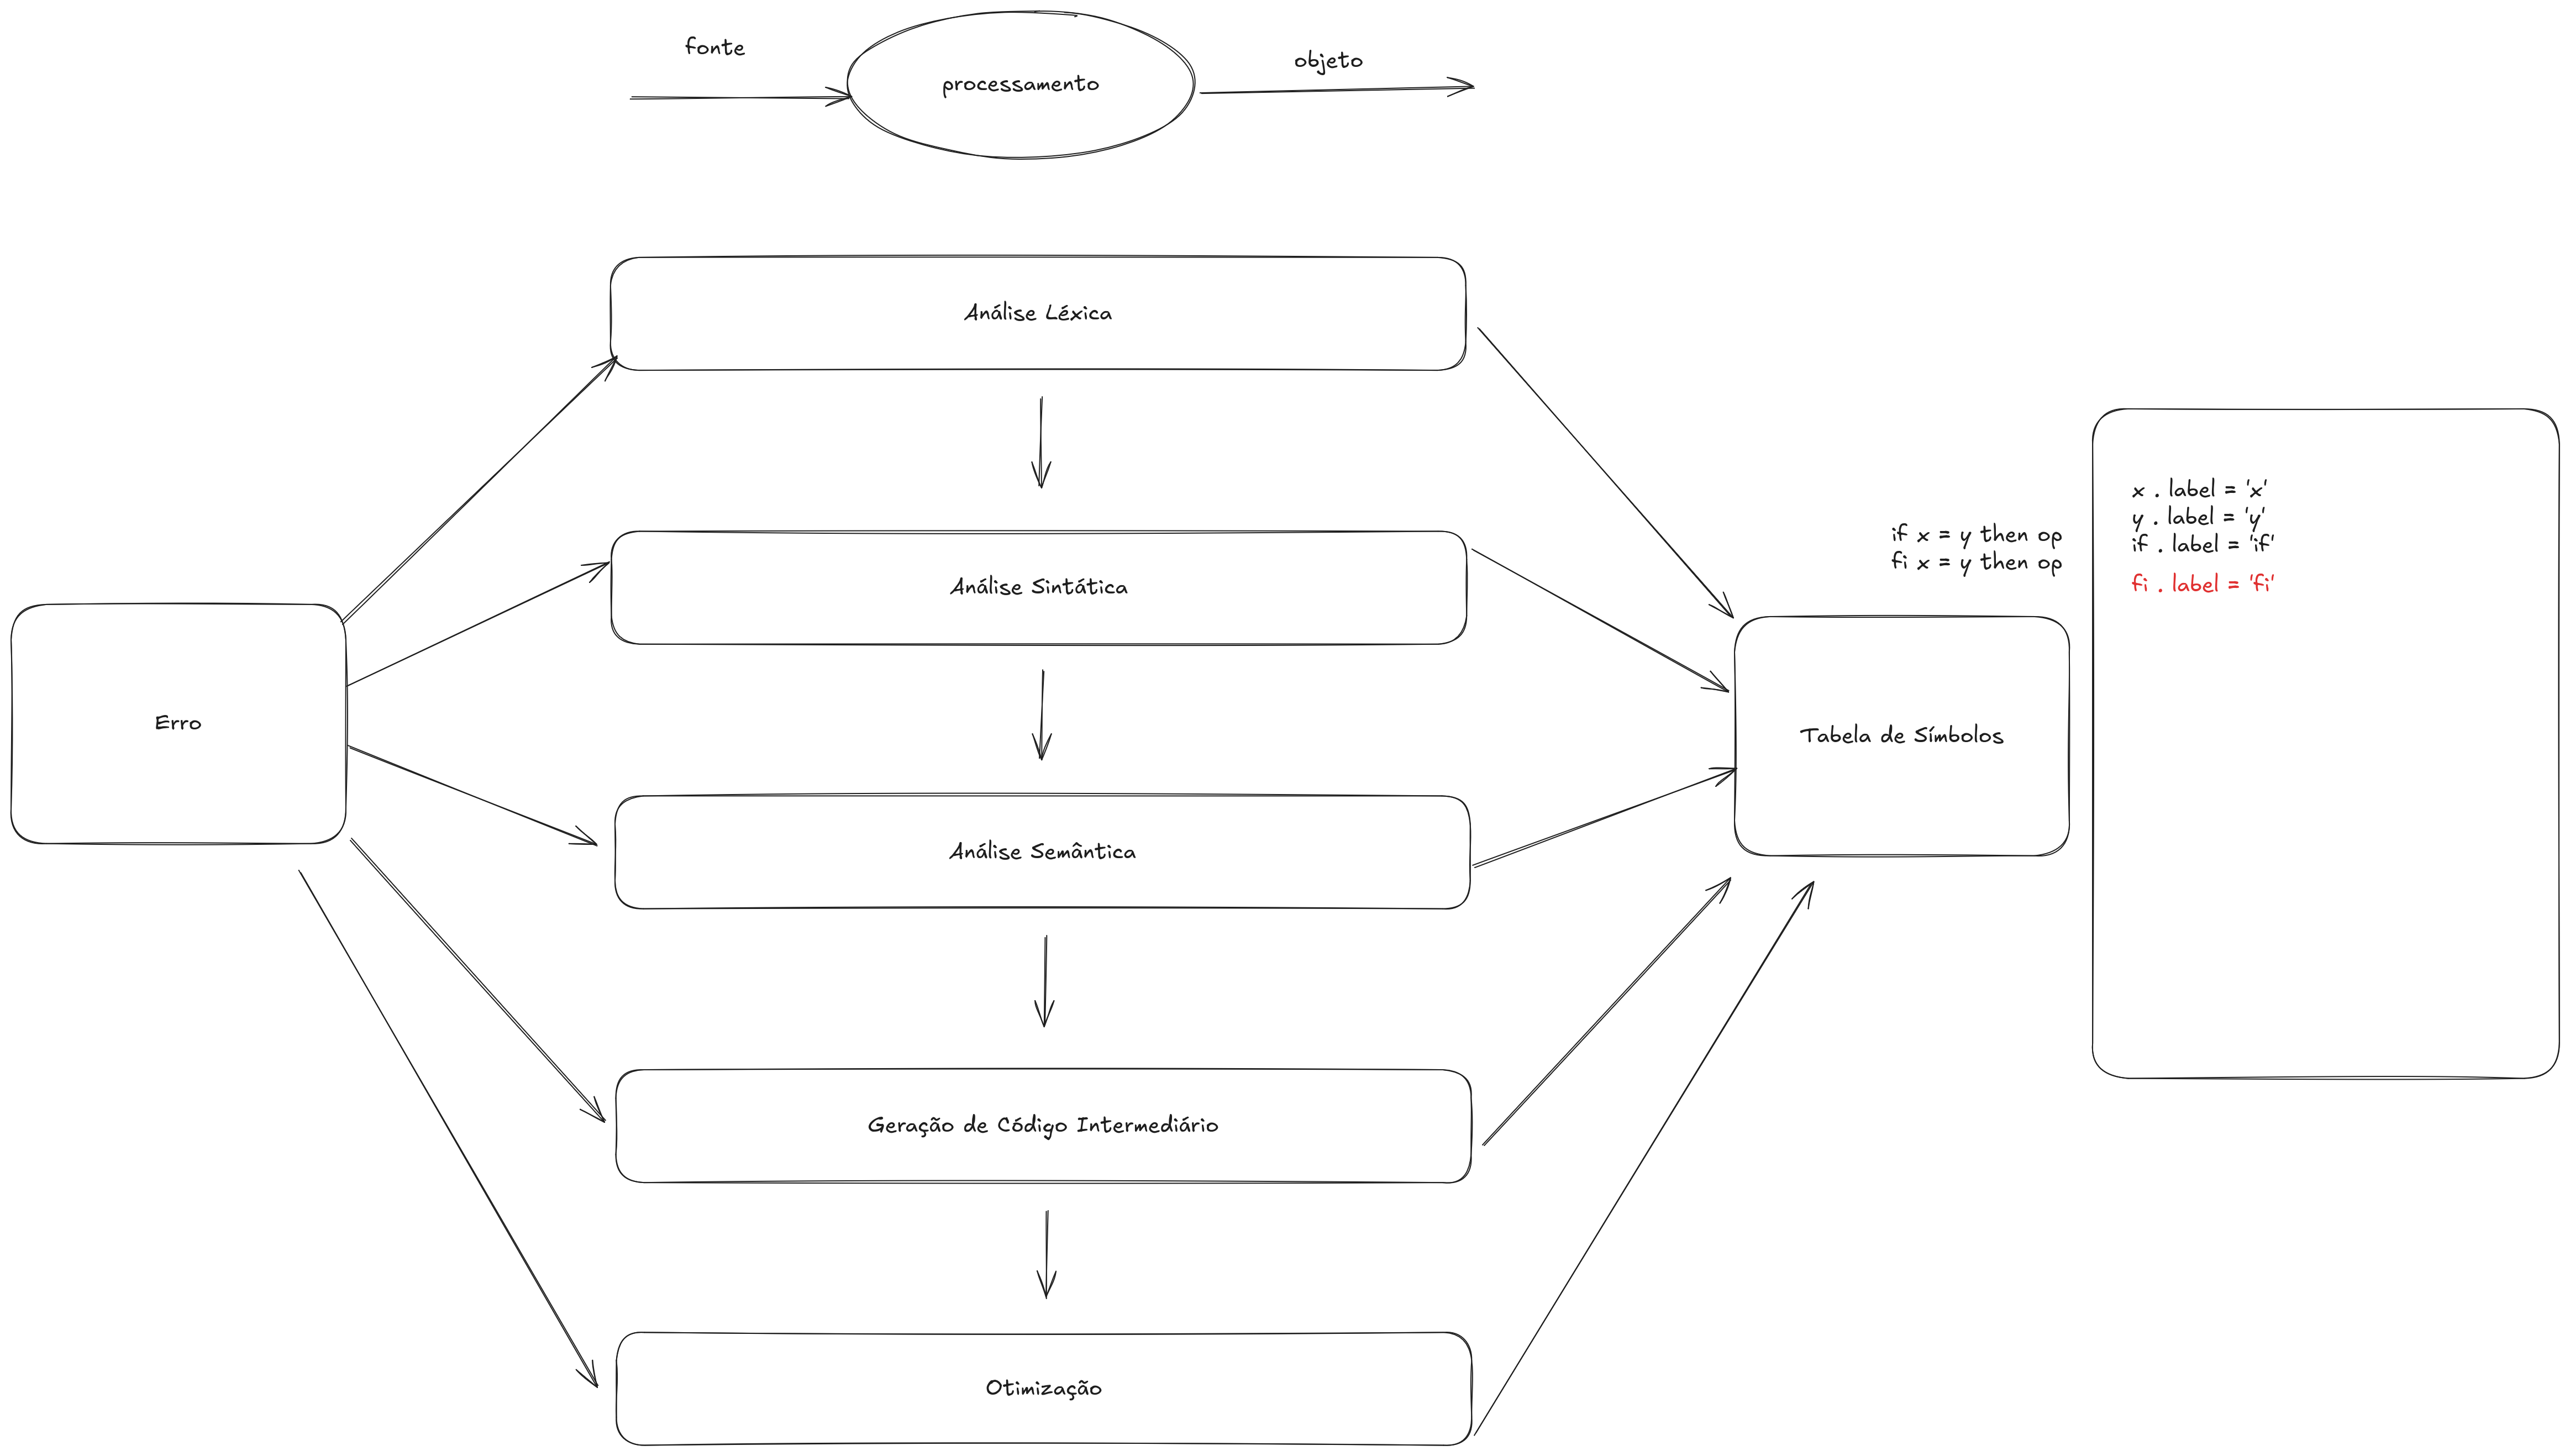
\includegraphics[scale=0.09]{images/aula-1.png}		
		\end{center}
		\subsection{Definição Formal da Gramática}
			\begin{enumerate}
				\item N: o conjunto de não terminais, ou variáveis.
				\item T: é o conjunto de terminais, ou alfabeto. Sendo que N e T são conjuntos distintos.
				\item P: é o conjunto distinto de produções, ou regras. \\ Sendo que:
				$P \subset (N \cup T)^{+} . (N \cup T)^{*}$
				\item S: é o símbolo não terminal que será o \textbf{símbolo inicial} de uma sentença %$S \to A \to \B \to C$...
			\end{enumerate}
	\section{Definição formal de gramática gerativa e derivação}
		A única operação da gramática gerativa é a \textbf{substituição}.
	\section{Análise Sintática}
	Uma estrutura sintática de uma \textbf{gramática} é determinada dessa maneira:
	$$<S> ::= <artigo><substantivo><verbo>$$
	$<artigo> ::= a$\\
	$<substantivo> ::= casa | coisa | lua$\\
	$<verbo> ::= caiu | saiu$\\
	
	Formalismo de Backus-Naur:
	\begin{itemize}
		\item $<substantivo> ::= casa$
		\item $<substantivo> ::= coisa$
		\item $<substantivo> ::= lua$
		\item $<verbo> ::= caiu$
		\item $<verbo> ::= saiu$
		\item $<artigo> ::= a$
	\end{itemize}
	Em seguida, temos a seguinte \textbf{produção}:\\
	$<S> \to <artigo><substantivo><verbo>$\\
	$<S>\to a <substantivo> <verbo>$\\
	$<S> \to a - casa<verbo>$\\
	$<S> \to a - casa- caiu$\\
	
	\newpage
	Exercício: 

	Altere a gramática acima para que possa acrescentar as seguintes frases:
	\begin{enumerate}
		\item o cão saiu
		\item o cofre fechou
		\item o gato saiu
		\item o gato caiu
	\end{enumerate}
	
		$$<S> ::= <artigo><substantivo><verbo>$$
	$<artigo> ::= a | o$\\
	$<substantivo> ::= casa | coisa | lua | cao | cofre | gato $\\
	$<verbo> ::= caiu | saiu | fechou$\\
	
	Correção:\\
	$ <S> ::= o<A>$\\
	$<A> ::= gato<B> | cao <C> | cofre <D>$\\
	$<B> ::= <C> | caiu$\\
%	$<B> ::= saiu | caiu$
	$<C> ::= saiu$\\
	$<D> ::= fechou$\\
	
%	\newpage
%	Exercício 2:\\
%	Considerando a gramática
%	$S::= o<A> | a<S2>$\\
%	$<A>::= gato<B> | cao <C> | cofre <D>$\\
%	$<B>::=<C>| caiu$\\
%	$<C>::=saiu$\\
%	$<D> ::= fechou$\\
%	$<S2> ::= <SUBS><VERBO>$\\
%	$<SUBS> ::= casa|coisa|lua$\\
%	$<VERBO>::= caiu|saiu$\\
%	
%	Altere a gramática para incluir as seguintes sentenças:
%	\begin{enumerate}
%		\item a casa fechou
%		\item o cofre caiu
%		\item o cofre saiu
%		\item o cão caiu
%		\item a lua saiu
%		\item a lua caiu
%		\item a coisa saiu
%		\item a coisa caiu
%		\item a casa saiu
%		\item a casa caiu
%		\item o cão saiu
%		\item o cofre fechou
%		\item o gato saiu
%		\item o gato caiu
%	\end{enumerate}
%		$S::= o<A> | a<S2>$\\
%	$<A>::= gato<B> | cao <W> | cofre <D>$\\
%	$<B>::=<C>| <X>$\\
%	$<W>::= <C>|<X>$
%	$<C>::=saiu$\\
%	$<X> ::= caiu$\\
%	$<Y>::= fechou$\\
%	$<D> ::= <C>| <Y>|<X>$\\
%	$<S2> ::= <SUBS><VERBO>$\\
%	$<SUBS> ::= casa|coisa|lua$\\
%	$<VERBO>::= <X>|<C>|<D>$\\
		\subsection{Derivação}
			Se $a \to b$, então a \textbf{produz} b\\
			se $a\to b\to c \to$...$\to z$ então $a \to ^* z$ e a produz z pelo \textbf{fecho derivativo}\\
			Então $a\to ^0 a$\\
			$a\to ^1 b$ se $a\to b$\\
%			$a \to ^{n+1} z$ se $a \to^n y e$
	\section{Hierarquia de Chomsky}
	Linguagens de tipo 3 (regulares) são resolvidas por gramáticas regulares
	
	O formalismo que resolve problemas de linguagens regulares é o \textbf{autômato finito}
	
	Linguagens do tipo 2 são resolvidas por gramáticas livre de contexto
	
	O formalismo que resolve é o \textbf{autômato de pilha}
	
	Gramáticas livre de contexto resolvem problemas do tipo 2 e do tipo 3.
	
	Linguages do tipo 1 são linguagens sensíveis ao contexto e são resolvitos por gramáticas irrestritas.
	
	\textbf{Máquinas irrestritas} resolvem problemas de linguagens do tipo 0 e do tipo 1.
	
	\subsection{Gramáticas Regulares (tipo 3)}
		Tem 3 formatos de produção possíveis, que é um não terminal que define o nome da regra e as produções podem ser nos formatos:\\
		$A::= a | aA| \epsilon$
	\subsection{Gramáticas Livres de Contexto}
		$A::=(N\cup T)^*$
	\subsection{Gramáticas Sensíveis ao Contexto}
		%Podemos definir o N que dá nome à regra não apenas como u
		Não inclui o Epsilon, portanto o menor tamanho das produções é 1\\
		$ |(N \cup T)^{+}|::= _{\leq} |(N \cup T)^*|$, o menor igual não se aplica na regra <S>. Ou seja, $<S> ::= \epsilon$
		
		$<S>$ não pode aparecer no lado direito de $P$.
		
	\subsection{Gramáticas Irrestritas}
		Não há restrição nenhuma, logo pode ser formado por qualquer concatenação:
		
		$(N\cup T)^+ ::= (N\cup T)^*$
	
\end{document}
